\subsection{Дискретизация уравнений JFO}

%% Блок 1: Вводный абзац
Задача~\eqref{eq:jfo_conservation}-\eqref{eq:jfo_complementarity}
является нелинейной комплементарной задачей: одновременно определяются
давление~$p$ и степень заполнения~$\vartheta$ при выполнении
неравенств.  Решение выполняется итерационно по стратегии активного
множества (active-set): на каждой итерации обновляется разбиение
области на зону полного заполнения и зону кавитации.  В настоящем
подразделе приводится общая схема алгоритма; детали дискретизации,
аппроксимации потоков и выбора солвера описаны в главе~3.

%% Блок 2: Сетка
Расчётная область покрывается равномерной сеткой:
\begin{equation}\label{eq:jfo_grid}
  \begin{aligned}
    &x_{1,i} = x_{1,s} + i\,\Delta x_1, \quad i = 0, \ldots, N_1 - 1, \\
    &x_{2,j} = x_{2,s} + j\,\Delta x_2, \quad j = 0, \ldots, N_2 - 1.
  \end{aligned}
\end{equation}

По периодическим направлениям применяются соответствующие условия
замыкания.  Операторы $\nabla$, $\nabla\!\cdot$ дискретизуются
в поверхностных координатах (подраздел~2.1.6); конкретные разностные
аппроксимации приведены в главе~3.

%% Блок 3: Консервативная дискретизация
Уравнение~\eqref{eq:jfo_conservation} записывается в дискретной
консервативной форме:
\begin{equation}\label{eq:jfo_discrete}
  \frac{(\vartheta h)_{i,j}^{n+1} - (\vartheta h)_{i,j}^{n}}{\Delta t}
  + \frac{F_{i+\frac{1}{2},j} - F_{i-\frac{1}{2},j}}{\Delta x_1}
  + \frac{G_{i,j+\frac{1}{2}} - G_{i,j-\frac{1}{2}}}{\Delta x_2}
  = 0,
\end{equation}
где $F$ и $G$ -- дискретные потоки по направлениям $x_1$ и $x_2$,
соответствующие напорному и переносному слагаемым
в~\eqref{eq:jfo_conservation}.  Потоки аппроксимируются так, чтобы
обеспечить консервативность (сохранение массы на дискретном уровне);
конкретный способ аппроксимации описан в главе~3.  В стационарной
постановке первый член в~\eqref{eq:jfo_discrete} опускается.

%% Блок 4: Идея active-set
На каждой итерации расчётная область разбивается на два множества:
\begin{itemize}
  \item зона полного заполнения: $p_{i,j} > p_{\mathrm{cav}}$,
    при этом $\vartheta_{i,j} = 1$; в этих узлах решается дискретная
    задача для давления~$p$ (уравнение Рейнольдса как частный случай
    при $\vartheta = 1$);
  \item зона кавитации (после проекции): $p_{i,j} = p_{\mathrm{cav}}$,
    при этом $0 \leq \vartheta_{i,j} < 1$; значение~$\vartheta$
    обновляется из дискретного уравнения
    сохранения~\eqref{eq:jfo_discrete}.
\end{itemize}
Переключение узлов между множествами продолжается до стабилизации
активного множества.

%% Блок 5: Псевдокод алгоритма
\begin{enumerate}
  \item Инициализация: $p^{(0)}_{i,j} = p_{\mathrm{cav}}$,
        $\vartheta^{(0)}_{i,j} = 1$.
  \item Цикл по $m = 0, 1, 2, \ldots$:
    \begin{enumerate}
      \item[2.1)] решить дискретную задачу для давления~$p$,
            полученную из~\eqref{eq:jfo_conservation}
            при фиксированном~$\vartheta^{(m)}$
            (и известном $(\vartheta h)^n$ в нестационарном случае);
      \item[2.2)] проекция:
            $p_{i,j} := \max(p_{i,j},\; p_{\mathrm{cav}})$;
      \item[2.3)] обновить активное множество: если
            $p_{i,j} > p_{\mathrm{cav}} + \varepsilon$ --
            полное заполнение ($\vartheta_{i,j} = 1$),
            иначе (после проекции
            $p_{i,j} = p_{\mathrm{cav}}$) -- кавитация
            (обновить $\vartheta_{i,j}$
            из~\eqref{eq:jfo_discrete});
      \item[2.4)] отсечка:
            $\vartheta_{i,j} := \min(1,\,\max(0,\,\vartheta_{i,j}))$;
      \item[2.5)] проверка сходимости.
    \end{enumerate}
  \item Выход: $p_{i,j}$, $\vartheta_{i,j}$.
\end{enumerate}
Здесь $\varepsilon$ -- малый численный допуск для устойчивого
определения активного множества.

\textit{Устойчивость и~сходимость алгоритма активного множества.}
Сходимость алгоритма активного множества в~задачах с~комплементарными ограничениями не~гарантирована в~общем случае. Для~задачи JFO, однако, можно указать условия, при~которых итерации сходятся. При~достаточно малом шаге сетки и~гладком поле зазора алгоритм обычно стабилизируется за~10--30 внешних итераций. Ключевым параметром является допуск~$\varepsilon$ в~шаге~2.3: при слишком малом~$\varepsilon$ возникают осцилляции активного множества (узлы на~границе кавитации попеременно переключаются между зонами), при~слишком большом~--- граница размывается и~нарушается точность условий комплементарности. Рекомендуемый диапазон: $\varepsilon$ порядка $10^{-6}$--$10^{-4}$ в~единицах характерного давления.

\textit{Чувствительность к~начальному приближению.}
Начальное приближение $p^{(0)} = p_{\mathrm{cav}}$, $\vartheta^{(0)} = 1$ (полное заполнение) является стандартным и~работоспособным, однако не~оптимальным с~точки зрения скорости сходимости. При~параметрических расчётах, когда вычисляется серия решений при~близких значениях параметра (например, различных эксцентриситетах или~нагрузках), существенного ускорения можно достичь методом тёплого старта: решение предыдущей задачи используется как~начальное приближение для~следующей. При~этом число внешних итераций сокращается в~несколько раз, поскольку активное множество уже близко к~истинному.

\textit{Преимущества консервативной дискретизации.}
Консервативная форма~\eqref{eq:jfo_discrete} обладает рядом важных свойств. Во-первых, она обеспечивает точный баланс масс на~каждой ячейке: суммарный поток через все~грани ячейки равен изменению накопленной массы за~шаг по~времени~--- это свойство выполняется точно, без~погрешности аппроксимации в~балансе. Во-вторых, консервативная схема устойчива к~разрывным полям~$\vartheta$, которые возникают на~границах кавитационных зон. Неконсервативные схемы (например, аппроксимация дивергентного оператора через центральные разности без~консервативных потоков на~гранях) могут давать локальные нарушения баланса масс вблизи границы кавитации, что проявляется в~физически нереалистичных осцилляциях давления и~степени заполнения. Консервативная схема свободна от~этого недостатка и~является предпочтительной при~расчёте подшипников с~множественными кавитационными зонами.

\textit{Устойчивость и~сходимость алгоритма активного множества.}
Сходимость алгоритма активного множества в~задачах с~комплементарными ограничениями не~гарантирована в~общем случае. Для~задачи JFO, однако, можно указать условия, при~которых итерации сходятся. При~достаточно малом шаге сетки и~гладком поле зазора алгоритм обычно стабилизируется за~10--30 внешних итераций. Ключевым параметром является допуск~$\varepsilon$ в~шаге~2.3: при слишком малом~$\varepsilon$ возникают осцилляции активного множества (узлы на~границе кавитации попеременно переключаются между зонами), при~слишком большом~--- граница размывается и~нарушается точность условий комплементарности. Рекомендуемый диапазон: $\varepsilon$ порядка $10^{-6}$--$10^{-4}$ в~единицах характерного давления.

\textit{Чувствительность к~начальному приближению.}
Начальное приближение $p^{(0)} = p_{\mathrm{cav}}$, $\vartheta^{(0)} = 1$ (полное заполнение) является стандартным и~работоспособным, однако не~оптимальным с~точки зрения скорости сходимости. При~параметрических расчётах, когда вычисляется серия решений при~близких значениях параметра (например, различных эксцентриситетах или~нагрузках), существенного ускорения можно достичь методом тёплого старта: решение предыдущей задачи используется как~начальное приближение для~следующей. При~этом число внешних итераций сокращается в~несколько раз, поскольку активное множество уже близко к~истинному.

\textit{Преимущества консервативной дискретизации.}
Консервативная форма~\eqref{eq:jfo_discrete} обладает рядом важных свойств. Во-первых, она обеспечивает точный баланс масс на~каждой ячейке: суммарный поток через все~грани ячейки равен изменению накопленной массы за~шаг по~времени~--- это свойство выполняется точно, без~погрешности аппроксимации в~балансе. Во-вторых, консервативная схема устойчива к~разрывным полям~$\vartheta$, которые возникают на~границах кавитационных зон. Неконсервативные схемы (например, аппроксимация дивергентного оператора через центральные разности без~консервативных потоков на~гранях) могут давать локальные нарушения баланса масс вблизи границы кавитации, что проявляется в~физически нереалистичных осцилляциях давления и~степени заполнения. Консервативная схема свободна от~этого недостатка и~является предпочтительной при~расчёте подшипников с~множественными кавитационными зонами.

%% Блок 6: Критерий сходимости
Итерации завершаются при выполнении условия
\[
  \max_{i,j}|p^{(m+1)}_{i,j} - p^{(m)}_{i,j}| < \varepsilon_p
\]
и стабилизации активного множества (ни один узел не переключился
между зонами).  При необходимости дополнительно контролируется
\[
  \max_{i,j}|\vartheta^{(m+1)}_{i,j} - \vartheta^{(m)}_{i,j}|
  < \varepsilon_\vartheta.
\]
Общая логика описанного алгоритма представлена
на рисунке~\ref{fig:jfo_algorithm}.

%% Рисунок: блок-схема алгоритма
\begin{figure}[!ht]
\centering
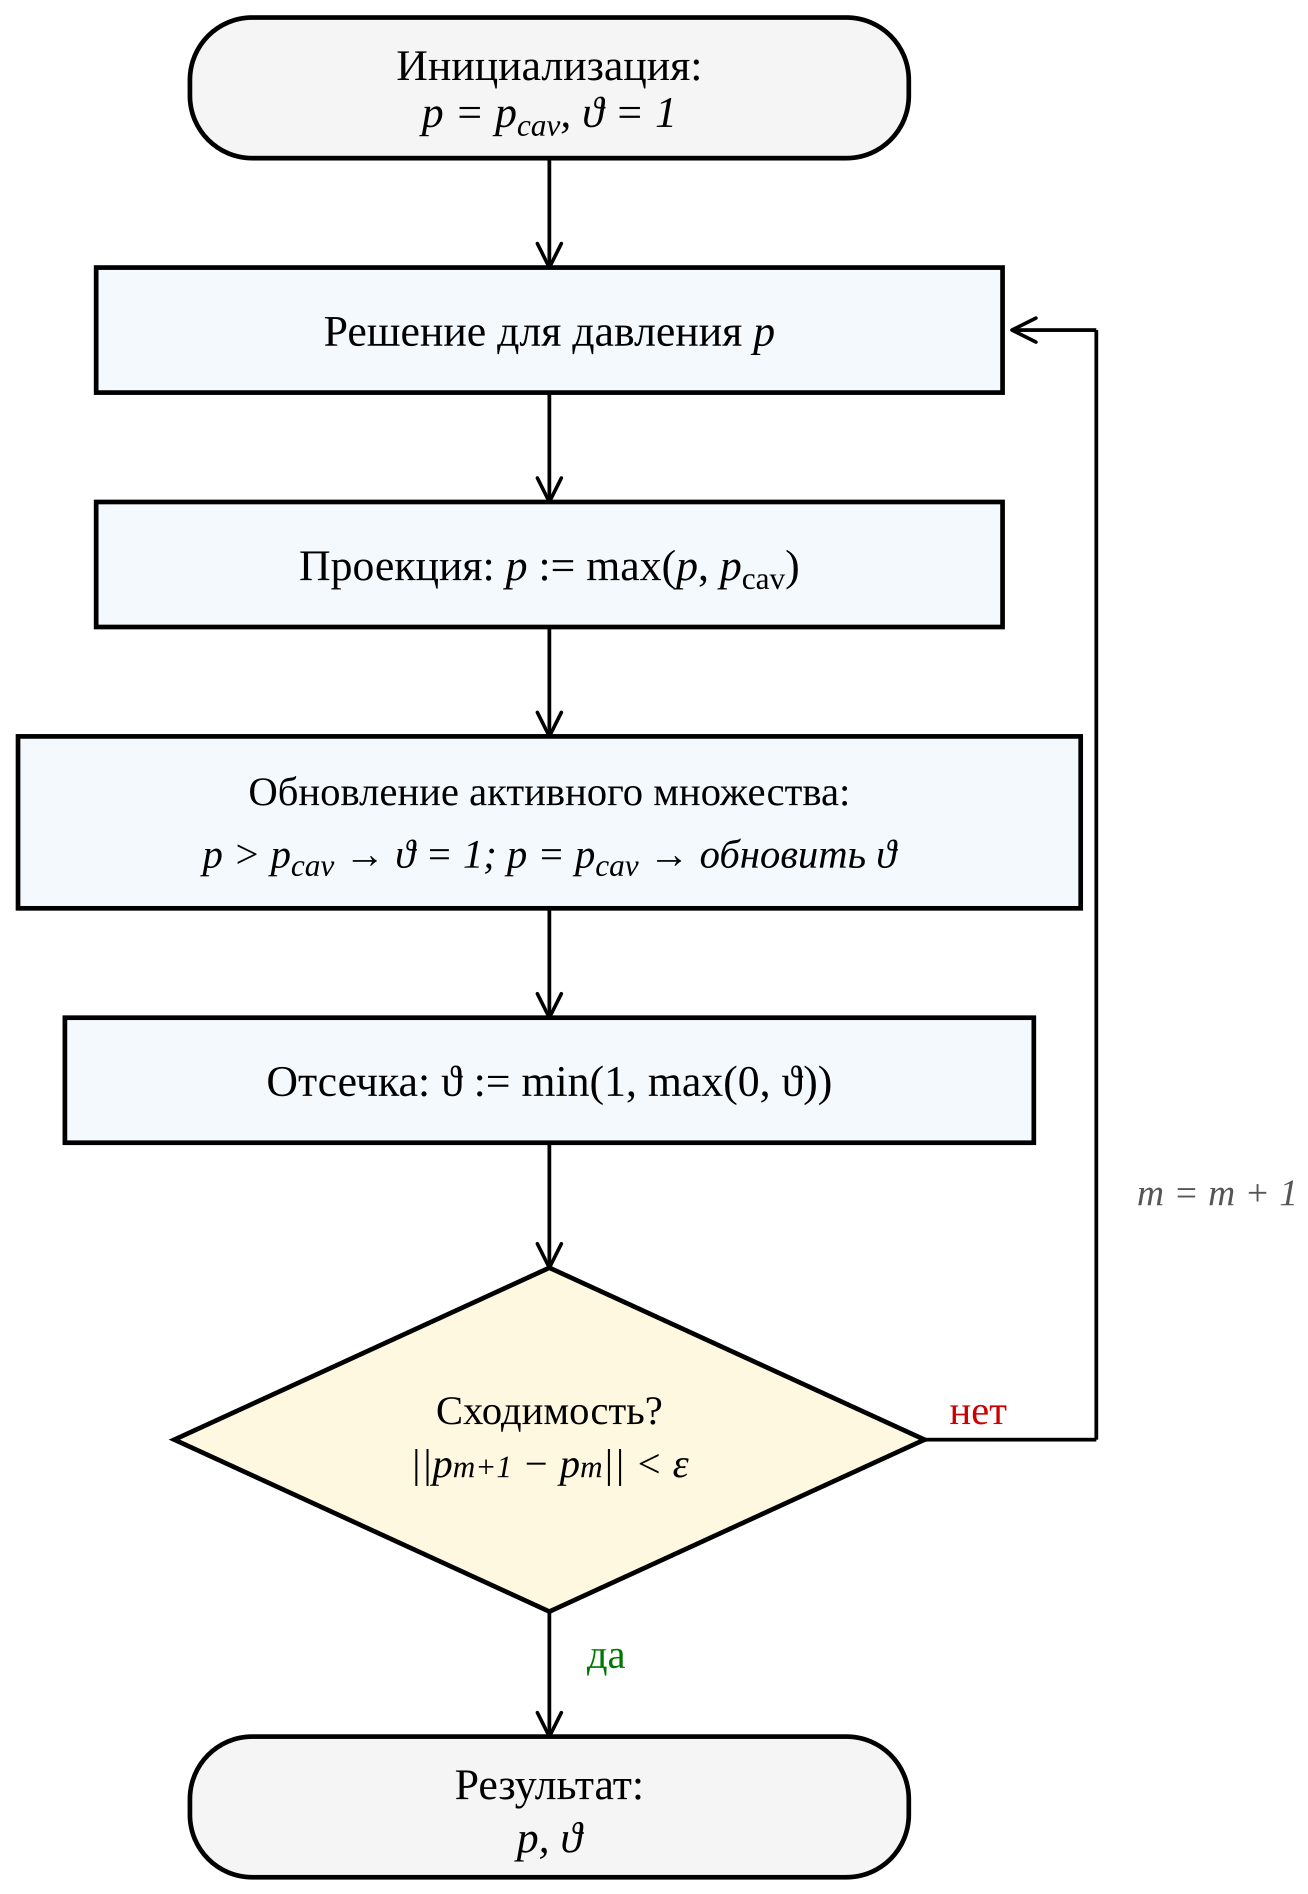
\includegraphics[width=\textwidth,height=0.9\textheight,keepaspectratio]{figures/ch02/fig_2_20.png}
\caption{Блок-схема итерационного алгоритма решения задачи JFO}
\label{fig:jfo_algorithm}
\end{figure}

%% Блок 8: Завершающий абзац
Описанная схема при консервативной аппроксимации потоков обеспечивает
массосохраняющее решение задачи кавитации~\cite{elrod1975,meng2017}
и применяется далее ко всем рассматриваемым постановкам (упорный,
радиальный и возвратно-поступательный подшипники).  Подробности
реализации, включая аппроксимацию потоков на гранях ячеек, выбор
солвера и диагностику баланса массы, приведены в главе~3.
